\documentclass[12pt,a4paper]{article}
\usepackage[latin1]{inputenc}
\usepackage[spanish]{babel}
\usepackage{amsmath}
\usepackage{amsfonts}
\usepackage[hidelinks]{hyperref}
\usepackage{amssymb}
\usepackage{graphicx}
\usepackage[left=2cm,right=2cm,top=2cm,bottom=2cm]{geometry}
\author{MEJORADA LOPEZ IVAN}
\title{ARREGLOS Y PARAMETROS DE LOS AMPLIFICADORES CLASE B}
\begin{document}
\maketitle

\includegraphics[width=17.5cm]{UPZMG_Prueba_1b.png} 
\newpage
\section{AMPLIFICADORES CLASE B}
 Los amplificadores de clase B se caracterizan por tener intensidad casi nula a trav\'es de sus transistores cuando no hay se\~nal en la entrada del circuito, por lo que en reposo el consumo es casi nulo.\\Un amplificador de potencia funciona en clase B cuando la polarizaci\'on de dc deja al transistor casi apagado de manera que el transistor se enciende cuando a este se le aplica una se\~nal en ac. Es decir que le transistor conducir\'a corriente solamente para una mitad de ciclo de la se\~nal.

Ahora para obtener una se\~nal de ciclo completo ser\'a necesario utilizar dos transistores y lograr que cada uno de ellos conduzca durante medios ciclos opuestos, y al tener esta operaci\'on combinada se obtiene un ciclo completo de se\~nal de salida.

Dado que una parte del circuito "empuja" a la se\~nal de arriba durante una mitad del ciclo y la otra parte "jala" la se\~nal hacia abajo durante la otra mitad del ciclo, el circuito por ende se denomina de contrafase circuito push-pull.
 \\
 \section{CARACTER\'ISTCAS}
 Se les denomina amplificador clase B, cuando el voltaje de polarizaci\'on y la m\'axima amplitud de la se\~nal entrante poseen valores que hacen que la corriente de salida circule durante el semiciclo de la se\~nal de entrada.

La caracter\'istica principal de este tipo de amplificadores es el alto factor de amplificaci\'on.

Amplificadores clase AB: Estos b\'asicamente son la mezcla de los dos anteriores. Cuando el voltaje de polarizaci\'on y la m\'axima amplitud de la se\~nal entrante poseen valores que hacen que la corriente de salida circule durante menos del ciclo completo y m\'as de la mitad del ciclo de la se\~nal de entrada, se les denomina: Amplificadores de potencia clase AB.
Dado que ocupa un lugar intermedio entre los de clase A y AB, cuando el voltaje de la se\~nal es moderado funciona como uno de clase A, cuando la se\~nal es fuerte se desempe\~na como uno de clase B, con una eficiencia y deformaci\'on moderadas.\\
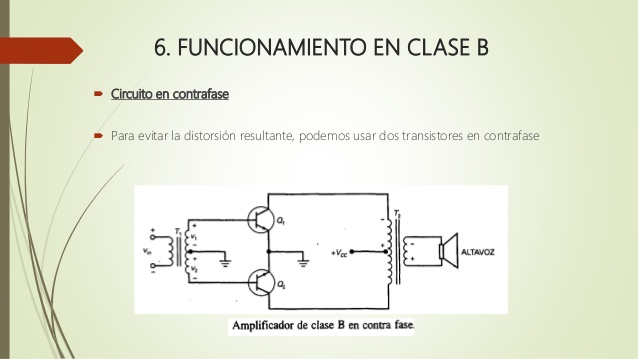
\includegraphics[width=18cm]{amplificadores-de-potencia-f-19-638.jpg} 
\newpage
\section{VENTAJAS}
*Posee bajo consumo en reposo.\\
*Aprovecha al m\'aximo la Corriente entregada por la fuente.\\
*Intensidad casi nula cuando est\'a en reposo.
\\
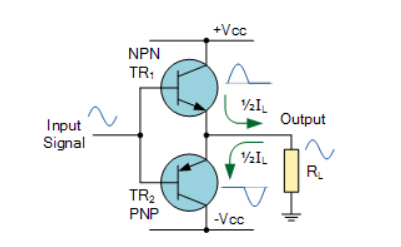
\includegraphics[width=18cm]{Amplificador clase AB.jpg} 
\section{DESVENTAJAS}
Producen arm\'onicos, y es mayor cuando no tienen los transistores de salida con las mismas caracter\'isticas t\'ecnicas, debido a esto se les suele polarizar de forma que se les introduce una peque\~na polarizaci\'on directa. Con esto se consigue desplazar las curvas y se disminuye dicha distorsi\'ong
\\
\section{APLICACION}
*Sistemas telef\'onicos,\\
*Transmisores de seguridad port\'atiles\\
*Sistemas de aviso, aunque no en audio.
\newpage
\section{Curvas de caracter\'isticas de salida de clase B
}
El amplificador de clase B tiene la gran ventaja sobre sus primos de amplificador de clase A en que ninguna corriente fluye a trav\'es de los transistores cuando están en estado de reposo (es decir, sin se\~nal de entrada), por lo tanto no se disipa potencia en los transistores de salida o transformador cuando no hay se\~nal presente a diferencia de las etapas de amplificador de Clase A que requieren un sesgo de base significativo, disipando as\'i gran cantidad de calor, incluso sin presencia de se\~nal de entrada\\Por lo tanto, la eficiencia total de conversi\'on del amplificador es mayor que la de la Clase A equivalente, alcanzando eficiencias tan altas como 70\%, lo que resulta en casi todos los tipos modernos de amplificadores push-pull operados en este modo Clase B.\\
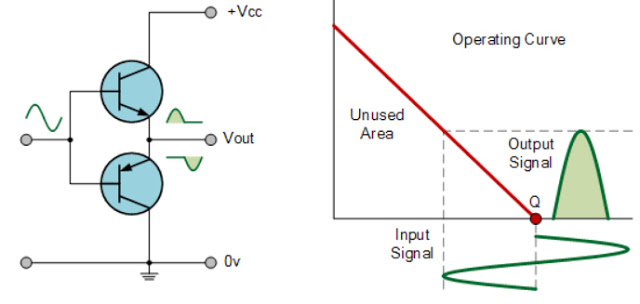
\includegraphics[width=15cm]{Amplificador de clase B.jpg} 
\\
\section{CONCLUCION}
Los amplificadores de clase B son muy preferidos sobre los dise\~nos de clase A para aplicaciones de alta potencia como amplificadores de potencia de audio y sistemas de PA. Al igual que el circuito amplificador de clase A, una forma de aumentar en gran medida la ganancia de corriente ( A i ) de un amplificador push-pull de Clase B es utilizar pares de transistores Darlington en lugar de transistores \'unicos en su circuito de salida.
  

\section{BIBLIOGRAFIA}
\url{https://www.ecured.cu/Amplificador_Clase_B}\\
\url{https://www.monografias.com/trabajos89/amplificador-potencia-clase-b/amplificador-potencia-clase-b.shtml}\\
\url{http://tutorialesdeelectronicabasica.blogspot.com/2018/06/amplificador-de-clase-b-y-amplificador.html}



\end{document}